\documentclass[a4paper]{article}

\usepackage[utf8]{inputenc}
\usepackage[polish]{babel}
\usepackage{polski}
\usepackage{listings}
\usepackage[margin=0.9in]{geometry}
\usepackage[usenames,dvipsnames]{xcolor}
\usepackage{lmodern}
\usepackage{pdfpages}

\author{Dorian Janiak, Marcin Ochman}
\title{Sprawozdanie projektowe z Robotów Mobilnych nr 1}


\begin{document}

\maketitle

\newpage

\tableofcontents
\listoffigures

\newpage

\section{Wstęp}

Sprawozdanie projektowe obejmuje postęp prac od 23.04.2015 do 14.04.2015, które zostały wykonane przez wszystkich członków grupy tj. \textit{Doriana Janiaka} oraz \textit{Marcina Ochmana}. Podczas tego okresu zrealizowano następujące rzeczy:
\begin{itemize}
	\item zostały rozpoczęte prace projektowe nad aplikacją uruchamianą na komputerze PC
	\item zostały rozpoczęte prace programistyczne nad aplikacją na komputer osobisty
	\item zostały stworzone diagramy dotyczące oprogramowania robota
\end{itemize}


\section{Opis wykonanych prac}

Poniżej zostały szczegółowo opisane prace, które wykonano na rzecz projektu.

\subsection{Prace projektowe nad aplikacją na PC}

Zostały stworzone dwa diagramy opisujące program, są one widoczne na rysunkach \ref{diagram_klas} oraz \ref{diagram_przypadkow_uzycia}. Pierwszy z nich to diagram klas, które będą wykorzystane w aplikacji. Drugi z nich to diagram przypadków użycia


\begin{figure}
\centering
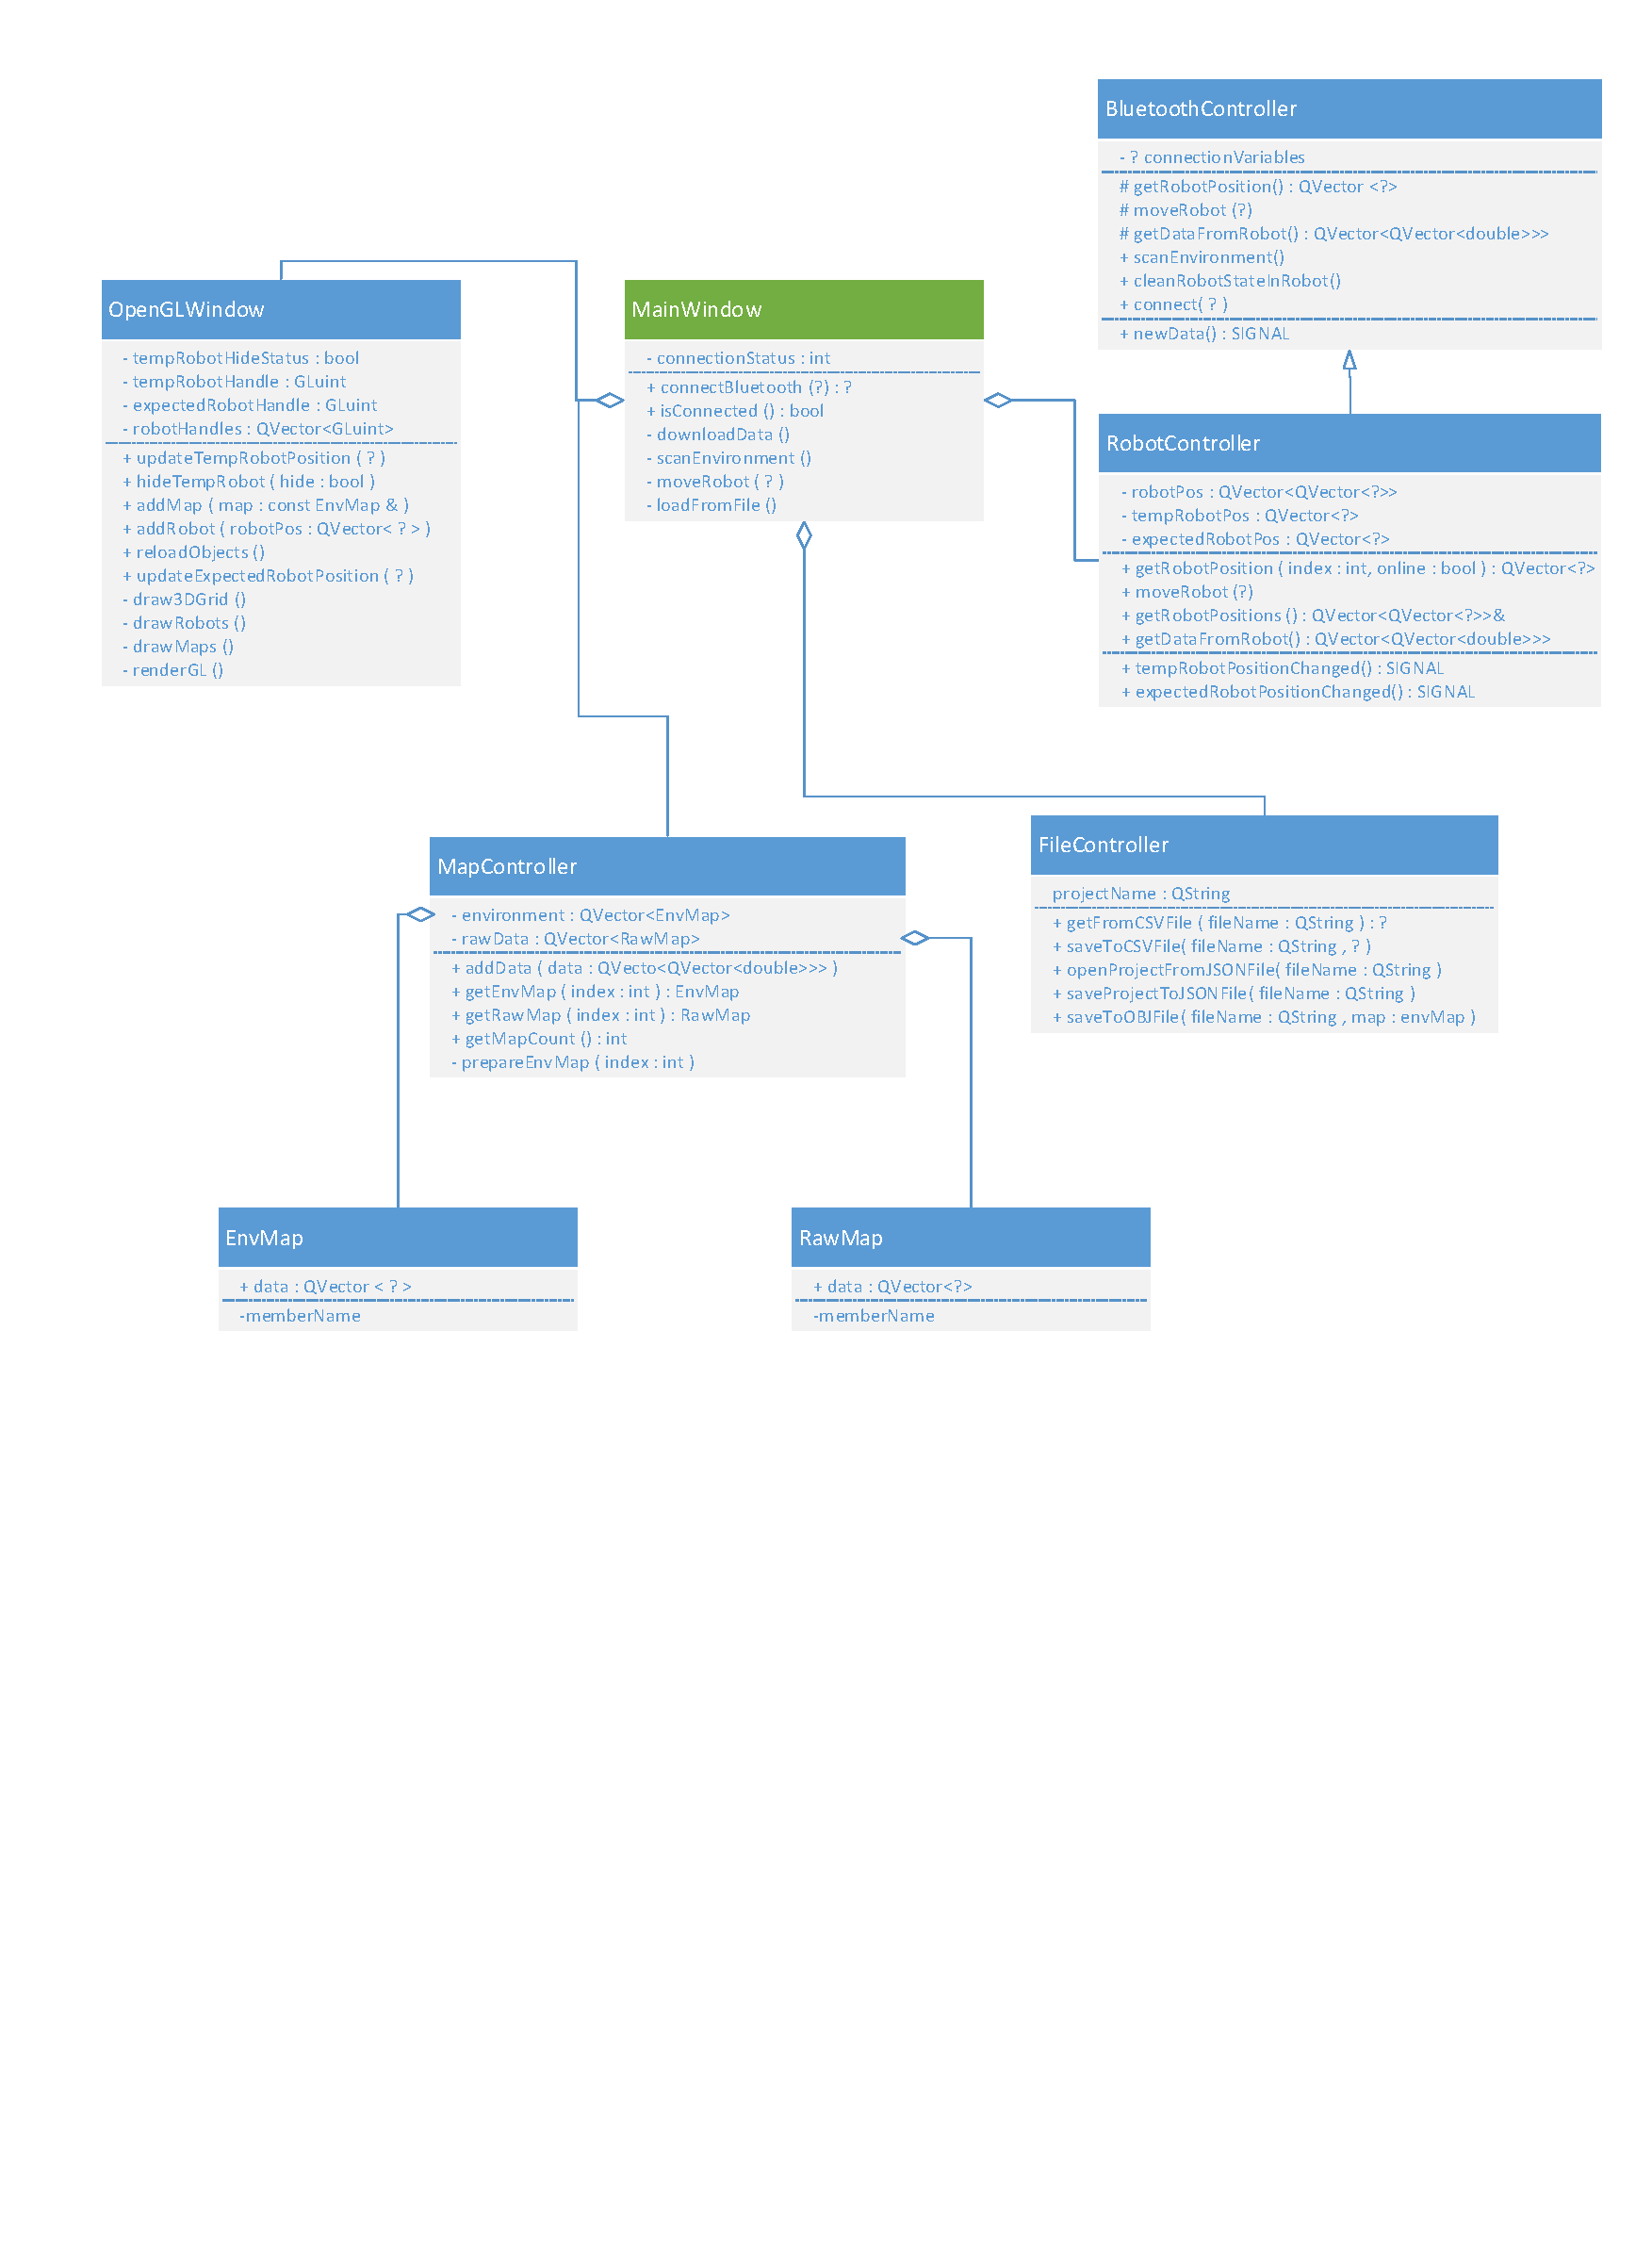
\includegraphics[height=0.9\paperheight, angle=90]{diagram_klas.pdf}
\caption{Diagram klas aplikacji PC}
\label{diagram_klas}
\end{figure}

\begin{figure}
\centering
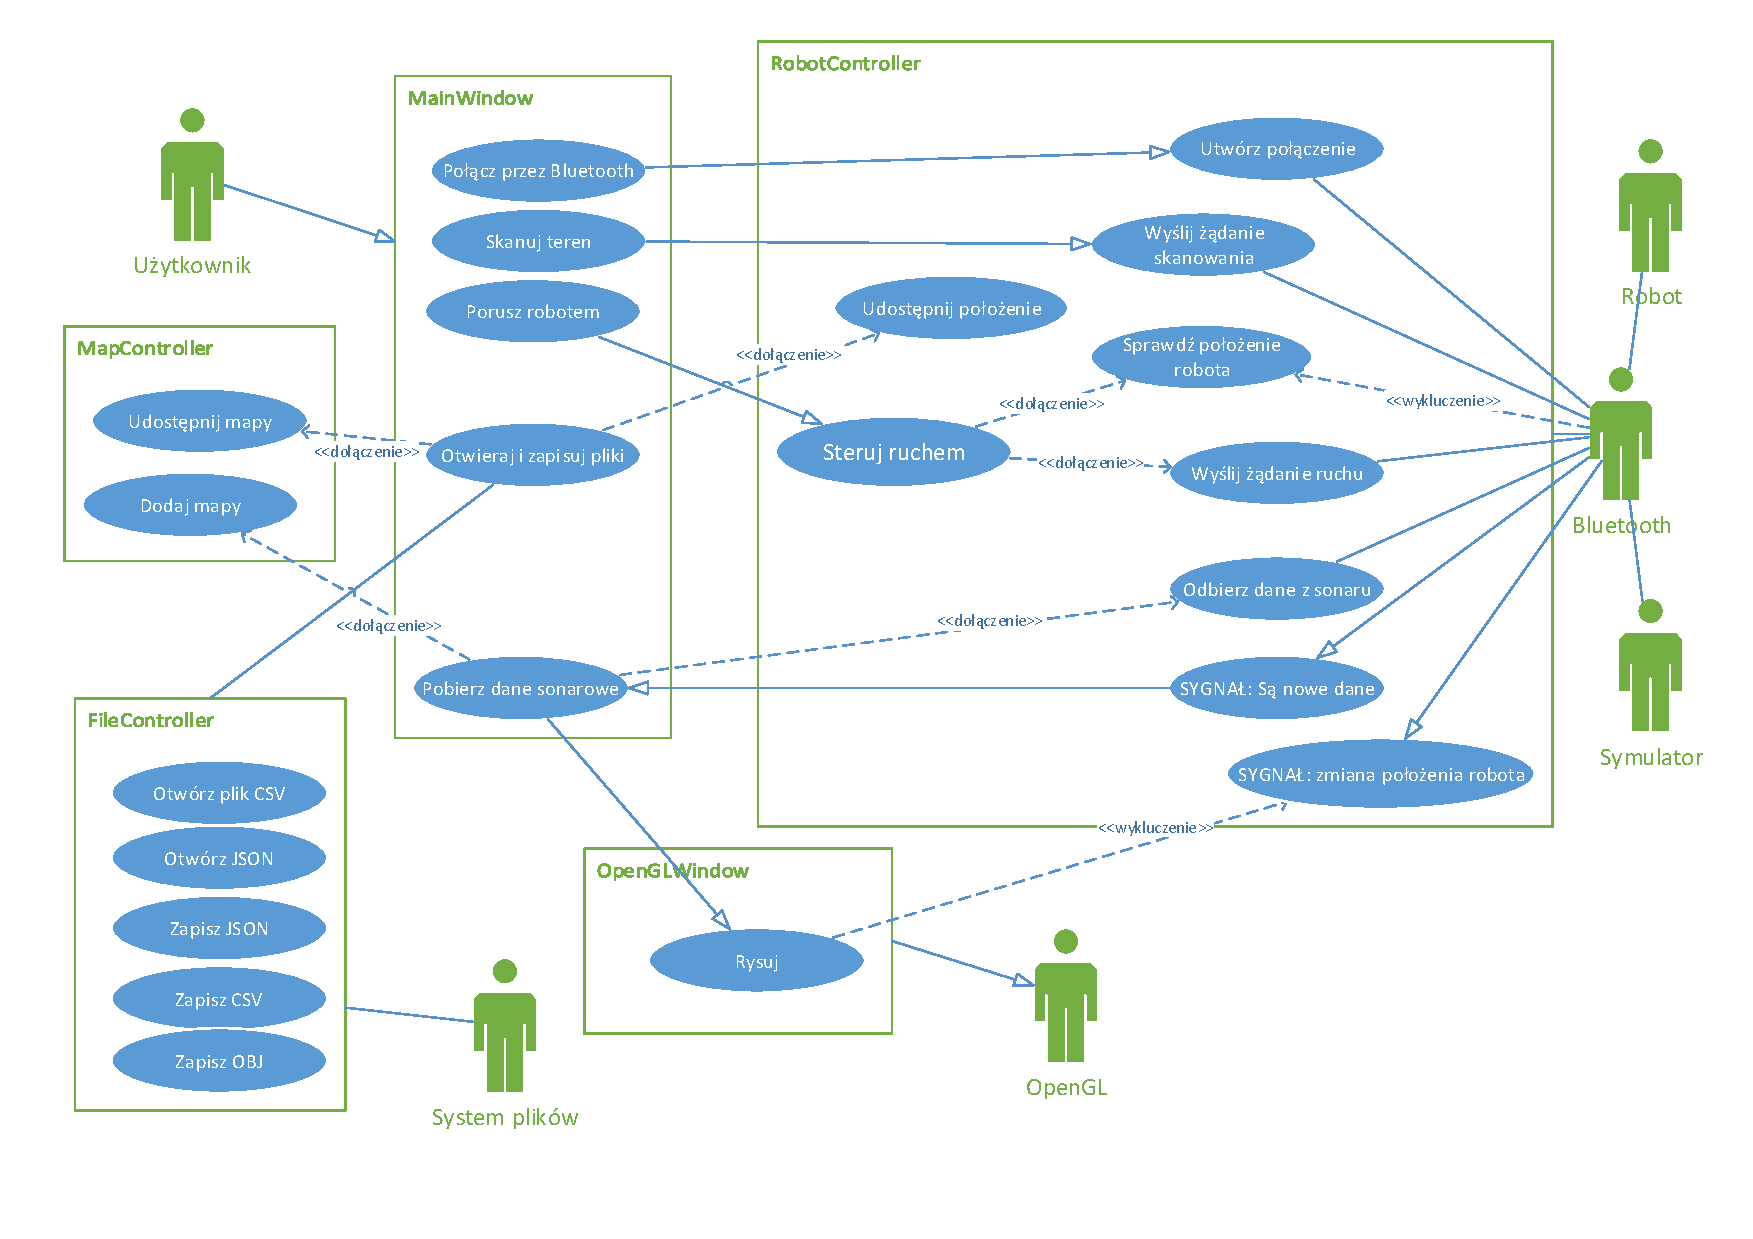
\includegraphics[height=0.55\paperheight, angle=90]{przypadki_uzycia.pdf}
\caption{Diagram przypadków użycia dla aplikacji PC}
\label{diagram_przypadkow_uzycia}
\end{figure}


\subsection{Prace programistyczne nad aplikacją PC}

Nasza aplikacja potrafi zainicjować środowisko 3D, narysować proste obiekty oraz stwarza możliwość poruszania oraz zmiany orientacji kamery. Jest to zalążek programu, dzięki któremu będziemy mogli wizualizować dane pochodzące z ultradźwiękowego czujnika odległości oraz ręcznie sterować robotem. Wszystko zostało zaimplementowane przy użyciu dwóch popularnych i uznanych bibliotek w języku \textit{C++}. Pierwsza z nich służy do tworzenia aplikacji okienkowych - \textit{Qt5}, druga z nich \textit{OpenGL} służy do generowania grafiki trójwymiarowej. Zrzut wyglądu programu został przedstawiony na rysunku \ref{aplikacja}.

\begin{figure}
\centering
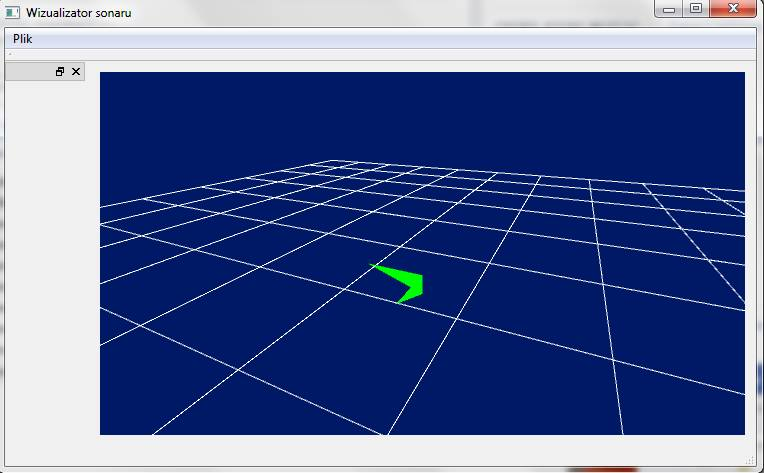
\includegraphics[width=\linewidth]{aplikacja}
\caption{Wygląd aplikacji}
\label{aplikacja}
\end{figure}


\subsection{Diagram dotyczący budowy robota oraz jego oprogramowania}

Na rysunku \ref{moduly_robota_pc} została przedstawiona komunikacja pomiędzy poszczególnymi modułami robota(zaznaczone na niebiesko). Diagram ten definiuje w jaki sposób będzie wyglądać sterowanie robotem oraz komunikacja pomiędzy komputerem osobistym. Widać, że za całe sterowanie będzie odpowiedzialny \textit{STM32}. To on będzie decydował jak mają poruszać się silniki, jak zostaną przetworzone informacje z enkoderów oraz czujnika ultradźwiękowego. Ostatecznie to on będzie odpowiedzialny za wysyłanie oraz odbieranie informacji i przetwarzanie komend przychodzących z komputera. Taka budowa definiuje w jaki sposób zostanie napisane oprogramowanie - każdy moduł sprzętowy będzie mieć własny moduł oprogramowania.

\begin{figure}
\centering
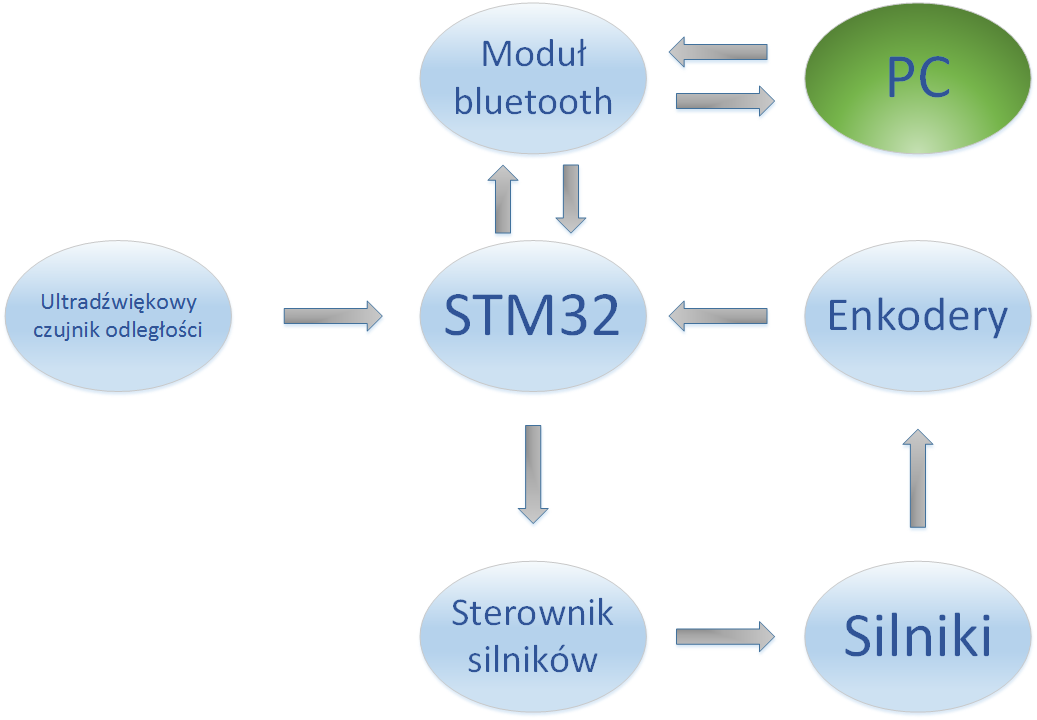
\includegraphics[width=\linewidth]{diagram_komunikacji_modulow_img}
\caption{Diagram przedstawiający moduły robota i PC oraz komunikację pomiędzy nimi}
\label{moduly_robota_pc}
\end{figure}


\section{Podsumowanie}

Zadania, które zostały wykonane pokrywają się z terminarzem zamieszczonym w poprzednim dokumencie dotyczącym założeń projektowych. Niepokojący może być fakt, że nie zostały jeszcze zakupione elementy do budowy robota, a co za tym idzie nie rozpoczęto prac nad jego budową. Jest to spowodowane bardzo ostrożnym wyborem elementów. Chcemy aby zakup był przemyślany, a każdy element poprawnie użyty. Pomimo opóźnienia w konstrukcji robota chcemy trzymać się planu i skończyć jego podwozie do 26 kwietnia. Kolejne etapy budowy zarówno aplikacji oraz robota nie powinny się opóźnić.

\section{Materiały źródłowe}

Naszym głównym źródłem informacji do stworzenia aplikacji były strony dokumentacji technicznej bibliotek - \textit{Qt5} oraz \textit{OpenGL}. Strony główne zostały zamieszczone poniżej:

\begin{itemize}
\item http://doc.qt.io/qt-5/reference-overview.html
\item https://www.opengl.org/documentation/
\end{itemize}

\end{document}